% memchar
%
%\documentclass[10pt,dvips]{article}
\documentclass[10pt,twocolumn]{article}
\usepackage[english]{babel}
\usepackage{epsfig}
%\usepackage{fancyheadings}
%\usepackage[T1]{fontenc}
%\usepackage[latin1]{inputenc}
%\usepackage{twocolumn}
%\usepackage{verbatim,moreverb,doublespace}
%\usepackage{rotate,lscape,dcolumn,array,rotating,latexsym}
%
%\input{epsf}
%
% for somebody (I forget now !)
%\textwidth 175mm
%\textheight 225mm
%\topmargin -4.5mm
%
% for somebody else (I also forget now !)
%\textwidth 6.6in 
%\textheight 239mm
%\topmargin -15mm
%\leftmargin -2.0in
%
% for (IEEE single-column format)
%\textwidth 6.875in
%\textheight 8.875in
%\topmargin -0.6in
%\oddsidemargin 0mm
%\evensidemargin 0mm
%
% for HPCA (IEEE two-column format)
\textwidth 6.5in
\textheight 8.875in
\topmargin -0.4in
%\oddsidemargin 0mm
%\evensidemargin 0mm
%
%
% some publishers want no page numbers for final print
%\pagestyle{empty}
%
\begin{document}
%
% going to 1mm here recoups some good space ! :-)
%\parskip 1mm
%\parskip 2mm
%
%
\title{Evaluating Memory Characteristics for Operand Bypass}
%
\author{
A. Khalafi, D. Morano, D.R. Kaeli\\
Northeastern University\\
{akhalafi, dmorano, kaeli}@ece.neu.edu\\
\and
A.K. Uht\\
University of Rhode Island\\ 
uht@ele.uri.edu
}
%
%
% some publishers do not want a data in the final print
\date{}
%
\maketitle
%
% uncomment the following for page with no page numbers (for IEEE)
%\thispagestyle{empty}
%
%
\begin{abstract}
%
We explore various intervals between memory loads and stores.
Distributions of three different types of access intervals
are defined and data is gathered on them using benchmarks.
The data on there access intervals serve to provide insight
about how a suitable microarchitecture might take advantage
of the memory access behavior in order to reduce the overhead
of general memory access transactions.
%
\end{abstract}
%
%
\vspace{-0.25in}
\section{Introduction}
\vspace{-0.15in}
%
This paper present data to characterize three types of
memory access intervals defined in terms of dynamic memory
instructions separating memory accesses.




%
%
\vspace{-0.25in}
\section{Register Access Statistics}
\vspace{-0.15in}
%
In this section, we show the register access statistics for
each of out ten benchmark programs.
The data is presented in three sets.
The first set of data is for register access-use intervals.
The second set of data is for register useful-lifetimes, and
the third is for register def-use intervals.

Data set one is shown in Figures \ref{fig:bzip2_rrint} 
through \ref{fig:craft_rrint}.
%
\begin{figure}
\centering
\epsfig{file=bzip2_rrint.eps,width=6.0in}
\caption{{\em Register Access-Use Intervals for BZIP2.} 
The density is shown on the left and the distribution is shown
on the right.
All intevals are measured in dynamic numbers of executed instructions.}
\label{fig:bzip2_rrint}
\end{figure*}
%





%
%
\vspace{-0.25in}
\section{Memory Access Statistics}
\vspace{-0.15in}
%
In this section, we show memory statistics for
the memory useful-lifetimes as well as for the def-use intervals.
Following are graphs of the cumulative data for :

\begin{enumerate}
\item One option is to dynamically follow
each output path and assign successively higher time tag values
to succeeding instructions.
\vspace{-0.15in}
\item The second option is to try to determine if the \textit{taken} outcome
of the branch joins with the \textit{not-taken} output instruction
stream.  If a join is determined, the instruction following
the \textit{not-taken} output path can be assigned a time value
one higher than the branch itself, while the first instruction
on the \textit{taken} path would be assigned whatever value
it would have gotten counting up from the first instruction
on the \textit{not-taken} path.
\end{enumerate}



.BL 10
.LI
memory access-use intervals (inter-reference gaps)
.LI
memory useful-lifetimes (def-last-useful-use intervals)
.LI
memory def-use intervals
.LE
.SP


Both a density and a distribution over the
associated intervals is shown.
The data is cumulative over all programs and memory variables
of each program.
.\"_
.\"_
.\"_
.\"_
.P
Figures \_MRINTDEN and \_MRINTDIS show the density and distribution
respectively for the memory reads over instruction intervals.
An access is defined as either a read or a write.
So an access-usage interval is the interval in instructions
from either a read or a write to the next read of the same
variable.  
There an instance of an access-usage for each memory
read in the executed program.
.DS
.\"_ file(page) h w pos off flags label
.BP mrintden.eps -1 6.0i c 0.0i a0
.EP
.SP 1
.FG "Cumulative Memory Access-Usage Density"
.TAG MRINTDEN
.DE
.\"_
.DS
.\"_ file(page) h w pos off flags label
.BP mrintdis.eps -1 6.0i c 0.0i a0
.EP
.SP 1
.FG "Cumulative Memory Access-Usage Distribution"
.TAG MRINTDIS
.DE
.\"_
.\"_
.\"_
.P
Figures \_MLIFEDEN and \_MLIFEDIS show the density and distribution
respectively for the memory writes over the useful-lifetime interval
as measured in instructions.
Our definition of \fIUseful-lifetime\fP 
(which is the same as that by Franklin and Sohi)
is the interval in dynamic instructions from a write of a variable
to the last useful read of the same variable.
There is an instance of a useful-lifetime associated with
each write of the executed programs.  However, it should be noted
that the present data does not include the last write for which
the last useful read has not yet been determined. 
This would seem to be more appropriate than assuming that the
last executed read of a variable was indeed the same useful read (since
it is unknown whether there are further reads afterwards).
.DS
.\"_ file(page) h w pos off flags label
.BP mlifeden.eps -1 6.0i c 0.0i a0
.EP
.SP 1
.FG "Cumulative Register Useful-Lifetime Density"
.TAG MLIFEDEN
.DE
.\"_
.DS
.\"_ file(page) h w pos off flags label
.BP mlifedis.eps -1 6.0i c 0.0i a0
.EP
.SP 1
.FG "Cumulative Memory Useful-Lifetime Distribution"
.TAG MLIFEDIS
.DE
.\"_
.\"_
.P
Figures \_MUSEDEN and \_MUSEDIS show the density and distribution
respectively for the memory reads over
intervals
as measured in instructions.
.DS
.\"_ file(page) h w pos off flags label
.BP museden.eps -1 6.0i c 0.0i a0
.EP
.SP 1
.FG "Cumulative Memory Def-Use Density"
.TAG MUSEDEN
.DE
.\"_
.DS
.\"_ file(page) h w pos off flags label
.BP musedis.eps -1 6.0i c 0.0i a0
.EP
.SP 1
.FG "Cumulative Memory Def-Use Distribution"
.TAG MUSEDIS
.DE
.\"_
.\"_
.\"_
.\"_





%
\begin{figure*}
\centering
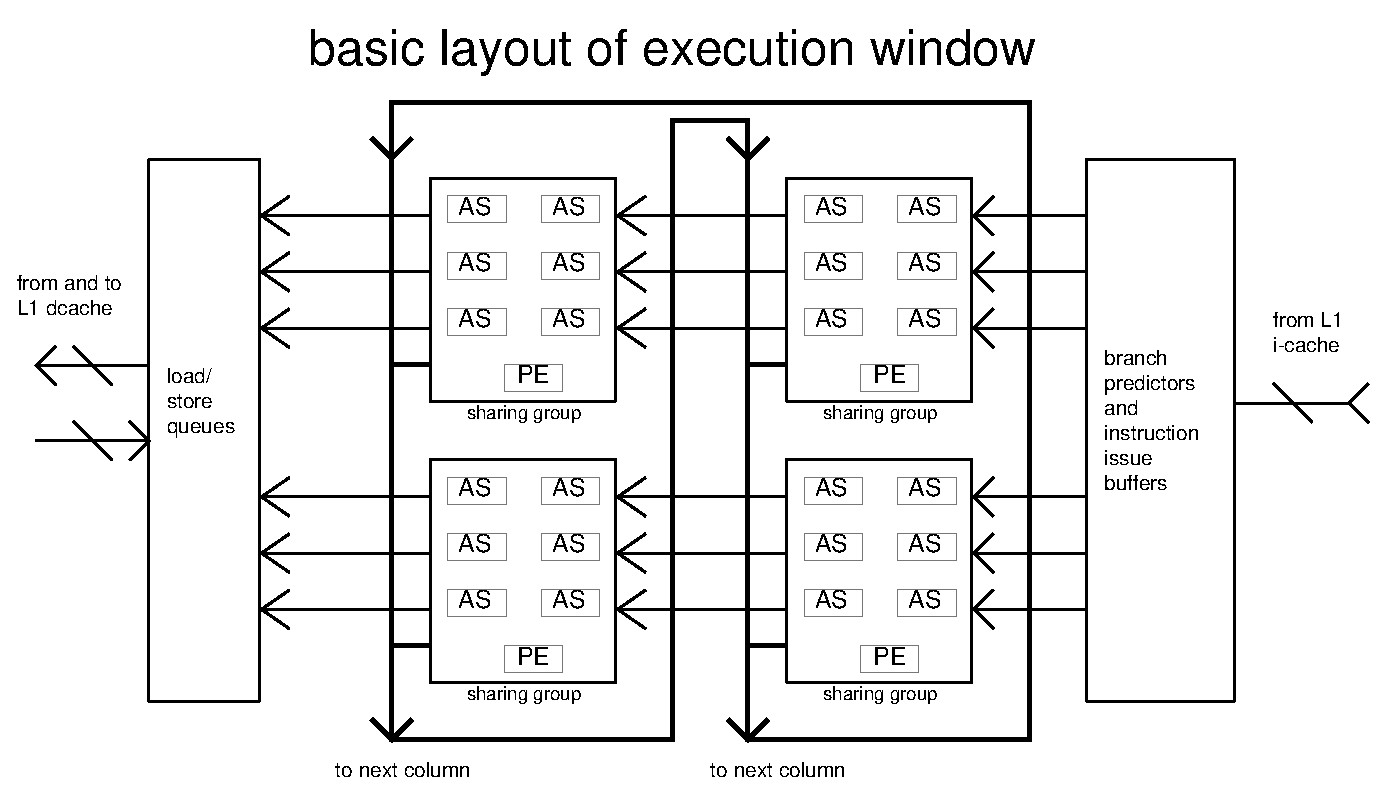
\epsfig{file=window.eps,width=4.0in}
\caption{{\em Execution Window.} Shown are four sharing groups
each with six active stations and one shared processing element.
There are six rows of ASes in each column of the entire arrangement.}
\label{fig:window}
\end{figure*}
%





%
%
\vspace{-0.25in}
\section{Summary}
\vspace{-0.15in}
%
We have presented a method for tracking and enforcing


%
\bibliographystyle{latex8}
\bibliography{memchar}
%
\end{document}
%
%
%
